% !TeX program = lualatex
% ================================================================
% Polish Tier 3 Vocabulary Version of FractionsDecimalsPercentagesRevision
%
% Generated by the server using the following settings:
%
%   language            Polish (pol)
%   text direction      left to right
%   font                Noto Serif
%   fallback font       Noto Serif
%   built from          latex/worksheets/revision/fractionsDecimalsPercentagesRevision.tex
%   vocabulary key      latex/worksheets/revision/fractionsDecimalsPercentagesRevision/L2/pol/fractionsDecimalsPercentagesRevision_polishKey.tex
%   tier 3 vocabulary   green   RGB 0 128 0
%   English text        black   RGB 0 0 0
%   Polish text         purple  RGB 112 48 160
%   layout macros       version 3
%
% Please don't edit any information in this comment block - the server
% compares it against the current settings and rebuilds this file when
% they differ, so changes here would be overwritten. However, feel free
% to make updates to the LaTeX below if you want to edit it.
% ================================================================

\documentclass[11pt,a4paper]{article}
% ================================================================
% Copied from the English sheet this was translated from, so that
% anything it sets up for itself still works here
% ================================================================
\usepackage[a4paper,top=14mm,bottom=14mm,left=15mm,right=15mm]{geometry}
\usepackage[T1]{fontenc}
\usepackage{amsmath}
\usepackage{amssymb}
\usepackage{array}
\usepackage{multicol}
\usepackage{tikz}
\usetikzlibrary{arrows.meta,decorations.pathreplacing}

% ================================================================
% Fractions, decimals and percentages: revision questions.
%
% Two pages of questions, in black and white, with a heading for each
% topic on the Maths Revision topic list in the same order. Each topic
% has a few short questions that start easy, with a diagram only where
% a question uses one, and the sheet ends with some problem solving.
% There are no key facts or worked examples on the sheet: the methods
% are in the worked solutions and the revision guide. Questions are
% numbered through the sheet so that the answer key and the worked
% solutions can refer to them.
% ================================================================

\pagestyle{empty}
\setlength{\parindent}{0pt}
\setlength{\parskip}{2pt}
\setlength{\columnsep}{9mm}

% A topic from the revision list.
\newcommand{\topic}[1]{\par\addvspace{9pt}{\bfseries #1}\par\nobreak\vspace{2pt}}

% Questions are numbered through the whole sheet.
\newcounter{qn}
\newcommand{\q}{\par\addvspace{5pt}\stepcounter{qn}\hangindent=1.6em\hangafter=1\noindent
  \makebox[1.6em][l]{\textbf{\theqn}}}

% \fracbars{<bars>}{<parts in each bar>}{<parts shaded>}{<bars in a row>}{<part width>}
\newcommand{\fracbars}[5]{%
  \begin{tikzpicture}[x=#5,y=4mm]
    \foreach \b in {1,...,#1}{%
      \pgfmathtruncatemacro{\fcr}{(\b-1)/#4}%
      \pgfmathtruncatemacro{\fcc}{mod(\b-1,#4)}%
      \foreach \p in {1,...,#2}{%
        \pgfmathtruncatemacro{\fck}{(\b-1)*#2+\p}%
        \pgfmathsetmacro{\fcx}{\fcc*(#2+0.8)+\p-1}%
        \pgfmathsetmacro{\fcy}{-\fcr*1.6}%
        \ifnum\fck>#3\relax
          \draw (\fcx,\fcy) rectangle ++(1,1);
        \else
          \draw[fill=black!15] (\fcx,\fcy) rectangle ++(1,1);
        \fi}}
  \end{tikzpicture}}

% \hundredgrid{<squares shaded>}{<square size>}: shaded row by row.
\newcommand{\hundredgrid}[2]{%
  \begin{tikzpicture}[x=#2,y=#2]
    \foreach \i in {0,...,99}{%
      \pgfmathtruncatemacro{\r}{\i/10}%
      \pgfmathtruncatemacro{\c}{mod(\i,10)}%
      \ifnum\i<#1\relax \fill[black!15] (\c,-\r) rectangle ++(1,1);\fi}
    \draw[step=1] (0,-9) grid (10,1);
  \end{tikzpicture}}

% Characters this language's font has not got are borrowed from another,
% rather than being silently dropped - see docs/translated-sheet-latex.md
\directlua{%
  if luaotfload and luaotfload.add_fallback then
    luaotfload.add_fallback("eallatinfallback",
      { "Noto Serif:mode=harf;" })
  else
    tex.error("this luaotfload is too old to register a fallback font")
  end
}
\usepackage[english]{babel}
\babelprovide[import]{polish}
\babelfont[polish]{rm}[Renderer=Harfbuzz, BoldFont={Noto Serif}, ItalicFont={Noto Serif}, BoldItalicFont={Noto Serif}, RawFeature={fallback=eallatinfallback}]{Noto Serif}
\babelfont[polish]{sf}[Renderer=Harfbuzz, BoldFont={Noto Serif}, ItalicFont={Noto Serif}, BoldItalicFont={Noto Serif}, RawFeature={fallback=eallatinfallback}]{Noto Serif}
\newcommand{\ealtext}[1]{\foreignlanguage{polish}{#1}}
\newcommand{\ealtextblock}[1]{{\raggedright\foreignlanguage{polish}{#1}\par}}
% ================================================================
% EAL layout helpers
% ================================================================
\usepackage{xcolor}

\definecolor{ealkeycolour}{RGB}{0,128,0}
\definecolor{ealenglish}{RGB}{0,0,0}
\definecolor{ealtwocolour}{RGB}{112,48,160}

\newsavebox{\ealboxen}
\newsavebox{\ealboxtr}
\newlength{\ealglosswd}
\newlength{\ealglossraise}
\setlength{\ealglossraise}{1.15em}

% a tier 3 word, in English and in translation alike
\newcommand{\ealkey}[1]{\textcolor{ealkeycolour}{#1}}
\newcommand{\ealkeytr}[1]{\textcolor{ealkeycolour}{\ealtext{#1}}}

% One translated word above one English word. Built from kernel
% primitives, never a tabular, which would break wherever the sheet
% loads array, booktabs or tabularx. The box is as wide as the wider of
% the two, so a long translation pushes its neighbours aside instead of
% overlapping them, and it claims its full height so a table row or a
% TikZ node makes room for it.
\newcommand{\ealgloss}[2]{%
  \sbox{\ealboxen}{\ealkey{#1}}%
  \sbox{\ealboxtr}{\small\textcolor{ealtwocolour}{\ealtext{#2}}}%
  \setlength{\ealglosswd}{\wd\ealboxen}%
  \ifdim\wd\ealboxtr>\ealglosswd\setlength{\ealglosswd}{\wd\ealboxtr}\fi
  \leavevmode
  \makebox[\ealglosswd][c]{%
    \makebox[0pt][c]{\usebox{\ealboxen}}%
    \makebox[0pt][c]{\raisebox{\ealglossraise}{\usebox{\ealboxtr}}}%
  }%
}

% opens up line spacing around a block of glosses, so the raised
% translations sit clear of the line above
\newenvironment{ealglossed}{\par\linespread{2.1}\selectfont\ignorespaces}{\par}

% a whole translated sentence above its English counterpart. block level,
% so it does not belong inside a tabular cell
\newcommand{\ealpara}[2]{%
  \par\addvspace{0.5\baselineskip}%
  {\color{ealtwocolour}\ealtextblock{#1}}%
  \penalty200
  {\color{ealenglish}#2\par}%
  \addvspace{0.5\baselineskip}%
}

\begin{document}
% Ragged right, without \raggedright, which would make \\ end the
% paragraph and lose the hanging indent of a question's later lines.
\setlength{\rightskip}{0pt plus 4em}

\begin{ealglossed}
{\Large\bfseries \ealgloss{Fractions}{ułamki}, \ealgloss{decimals}{ułamki dziesiętne} and \ealgloss{percentages}{procenty}}\hfill{\large Revision questions}\par
\end{ealglossed}
\vspace{2pt}\hrule\vspace{4pt}

\begin{multicols}{2}

% ----------------------------------------------------------------
\begin{ealglossed}
\topic{\ealgloss{Simplifying}{Upraszczanie} \ealgloss{fractions}{ułamków}}
\q What \ealgloss{fraction}{ułamek} of the bar is shaded? Give your answer in its \ealgloss{simplest form}{najprostszej postaci}.\\[4pt]
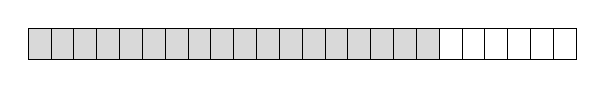
\begin{tikzpicture}[x=2.9mm,y=4mm]
  \fill[black!15] (0,0) rectangle (18,1);
  \foreach \i in {0,...,23}{\draw (\i,0) rectangle ++(1,1);}
\end{tikzpicture}
\q \ealgloss{Simplify}{Uprość}\quad (a) $\dfrac{12}{16}$\qquad (b) $\dfrac{30}{45}$\qquad (c) $\dfrac{84}{120}$
\end{ealglossed}

% ----------------------------------------------------------------
\begin{ealglossed}
\topic{Ordering \ealgloss{fractions}{ułamków}}
\q Write in order, smallest first.\\[2pt]
(a) $\dfrac34,\ \dfrac58,\ \dfrac7{12}$\qquad (b) $\dfrac45,\ \dfrac7{10},\ \dfrac34,\ \dfrac{13}{20}$
\q Ella eats $\frac38$ of a pizza. Sam eats $\frac25$ of an identical pizza. Who eats more?
\end{ealglossed}

% ----------------------------------------------------------------
\begin{ealglossed}
\topic{\ealgloss{Mixed numbers}{liczby mieszane} and \ealgloss{improper fractions}{ułamki niewłaściwe}}
\q Write the shaded amount as\\
(a) a \ealgloss{mixed number}{liczba mieszana}\qquad (b) an \ealgloss{improper fraction}{ułamek niewłaściwy}.\\[4pt]
\fracbars{3}{4}{11}{3}{4.4mm}
\q (a) Write $5\frac23$ as an \ealgloss{improper fraction}{ułamek niewłaściwy}.\\
(b) Write $\frac{31}6$ as a \ealgloss{mixed number}{liczba mieszana}.
\end{ealglossed}

% ----------------------------------------------------------------
\begin{ealglossed}
\topic{Adding and subtracting \ealgloss{fractions}{ułamków}}
\q (a) $\dfrac13+\dfrac15$\qquad (b) $\dfrac34-\dfrac27$\qquad (c) $\dfrac56+\dfrac38$
\q Jack spends $\frac14$ of his money on a game and $\frac25$ of it on clothes. What \ealgloss{fraction}{ułamek} of his money is left?
\end{ealglossed}

% ----------------------------------------------------------------
\begin{ealglossed}
\topic{One number as a \ealgloss{percentage}{procent} of another}
\q Write as a \ealgloss{percentage}{procent}.\\
(a) 12 out of 50\qquad (b) 27 out of 60\\
(c) 35\,cm out of 2\,m
\q Priya scores 34 out of 40 in a test. Leo scores 41 out of 50. Who did better?
\end{ealglossed}

% ----------------------------------------------------------------
\begin{ealglossed}
\topic{\ealgloss{Percentages}{procenty} without a calculator}
\q Find\quad (a) 10\% of 470\qquad (b) 50\% of 86\\
(c) 1\% of 650\qquad (d) 15\% of 360
\q A £45 jacket is reduced by 20\% in a sale. What is the sale price?
\end{ealglossed}

% ----------------------------------------------------------------
\columnbreak
\begin{ealglossed}
\topic{Converting between \ealgloss{fractions}{ułamkami}, \ealgloss{decimals}{ułamkami dziesiętnymi} and \ealgloss{percentages}{procentami}}
\q Write the shaded part of the grid as a \ealgloss{fraction}{ułamek} in its \ealgloss{simplest form}{najprostszej postaci}, as a \ealgloss{decimal}{ułamek dziesiętny} and as a \ealgloss{percentage}{procent}.\\[4pt]
\hundredgrid{36}{2.2mm}
\q Copy and complete the table.\\[4pt]
{\renewcommand{\arraystretch}{3}%
\begin{tabular}{|c|c|c|}\hline
\ealgloss{Fraction}{ułamek} & \ealgloss{Decimal}{ułamek dziesiętny} & \ealgloss{Percentage}{procent}\\\hline
$\frac35$ & & \\\hline
 & 0.45 & \\\hline
 & & 4\%\\\hline
\end{tabular}}
\end{ealglossed}

% ----------------------------------------------------------------
\begin{ealglossed}
\topic{Ordering \ealgloss{fractions}{ułamków}, \ealgloss{decimals}{ułamków dziesiętnych} and \ealgloss{percentages}{procentów}}
\q Write in order, smallest first.\\
(a) 0.4,\ \ $\frac38$,\ \ 41\%\qquad (b) $\frac13$,\ \ 0.3,\ \ 33\%
\q Shop A takes $\frac13$ off its prices. Shop B takes 30\% off. Shop C takes 0.35 of the price off. Which shop gives the biggest discount?
\end{ealglossed}

% ----------------------------------------------------------------
\begin{ealglossed}
\topic{\ealgloss{Fractions}{ułamki} of amounts}
\q Use the \ealgloss{bar model}{modelu słupkowego} to find $\frac35$ of 60.\\[4pt]
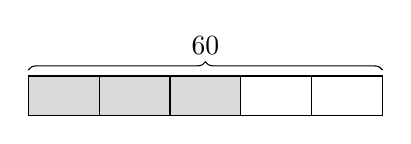
\begin{tikzpicture}[x=9mm,y=5mm]
  \fill[black!15] (0,0) rectangle (3,1);
  \foreach \i in {0,...,4}{\draw (\i,0) rectangle ++(1,1);}
  \draw[decorate,decoration={brace,amplitude=3pt}] (0,1.15) -- (5,1.15) node[midway,above=2pt] {60};
\end{tikzpicture}
\q (a) Without a calculator, find $\frac38$ of 64.\\
(b) With a calculator, find $\frac79$ of 504.
\q A school has 840 pupils. $\frac37$ of them have school dinners. How many pupils do not have school dinners?
\end{ealglossed}

% ----------------------------------------------------------------
\begin{ealglossed}
\topic{\ealgloss{Percentages}{procenty} of amounts}
\q Without a calculator, find\\
(a) 35\% of 140\qquad (b) 12.5\% of 64
\q With a calculator, find\\
(a) 23\% of 85\qquad (b) 4.5\% of £2400
\end{ealglossed}

% ----------------------------------------------------------------
\begin{ealglossed}
\topic{\ealgloss{Percentage change}{zmiana procentowa}}
\q Find the \ealgloss{percentage change}{zmianę procentową}.\\
(a) 50\,kg to 62\,kg\qquad (b) £80 to £68
\q A car bought for £12\,000 is sold two years later for £9000. Find the \ealgloss{percentage}{procentowy} decrease.
\end{ealglossed}

\end{multicols}

\newpage

\begin{multicols}{2}

% ----------------------------------------------------------------
\begin{ealglossed}
\topic{\ealgloss{Simple interest}{procent prosty}}
\q £500 is invested at 2\% \ealgloss{simple interest}{procentu prostego} per year. Copy and complete the table.\\[4pt]
{\renewcommand{\arraystretch}{1.5}%
\begin{tabular}{|l|c|c|c|c|c|}\hline
Year & 0 & 1 & 2 & 3 & 4\\\hline
Balance (£) & 500 & \hspace{6mm} & \hspace{6mm} & \hspace{6mm} & \hspace{6mm}\\\hline
\end{tabular}}
\q Amy invests £800 at 5\% \ealgloss{simple interest}{procentu prostego} per year. After how many years will she have £1000?
\end{ealglossed}

% ----------------------------------------------------------------
\begin{ealglossed}
\topic{Calculating with \ealgloss{mixed numbers}{liczbami mieszanymi} and \ealgloss{negatives}{ujemnymi}}
\q (a) $1\dfrac23+2\dfrac14$\qquad (b) $4\dfrac15-1\dfrac12$\qquad (c) $1\dfrac12\times2\dfrac23$
\q (a) $3\dfrac34\div1\dfrac14$\qquad (b) $-\dfrac23\times\dfrac9{10}$\\[4pt]
(c) $-1\dfrac14\div\left(-\dfrac58\right)$
\end{ealglossed}

% ----------------------------------------------------------------
\begin{ealglossed}
\topic{Word problems with \ealgloss{mixed numbers}{liczbami mieszanymi}}
\q A plank is $5\frac14$\,m long. A piece $2\frac23$\,m long is cut off. How long is the piece that is left?\\[4pt]
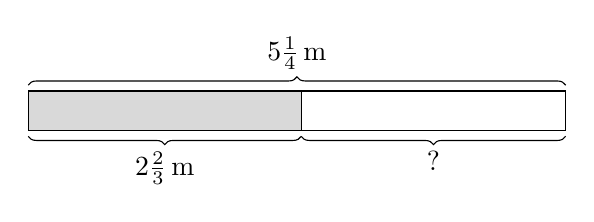
\begin{tikzpicture}[x=13mm,y=5mm]
  \fill[black!15] (0,0) rectangle (2.667,1);
  \draw (0,0) rectangle (5.25,1) (2.667,0) -- (2.667,1);
  \draw[decorate,decoration={brace,amplitude=3pt}] (0,1.15) -- (5.25,1.15) node[midway,above=2pt] {$5\frac14$\,m};
  \draw[decorate,decoration={brace,amplitude=3pt,mirror}] (0,-0.15) -- (2.667,-0.15) node[midway,below=2pt] {$2\frac23$\,m};
  \draw[decorate,decoration={brace,amplitude=3pt,mirror}] (2.667,-0.15) -- (5.25,-0.15) node[midway,below=2pt] {?};
\end{tikzpicture}
\q How many $\frac13$ litre glasses can be completely filled from a jug holding $2\frac34$ litres?
\q A rectangular garden is $6\frac12$\,m long and $3\frac13$\,m wide. Find its \ealgloss{area}{pole}.
\end{ealglossed}

% ----------------------------------------------------------------
\begin{ealglossed}
\topic{\ealgloss{Recurring decimals}{ułamki okresowe} to \ealgloss{fractions}{ułamków}}
\q Copy and complete to write $0.\dot4$ as a \ealgloss{fraction}{ułamek}.\\[3pt]
\begin{tabular}{@{}r@{\;=\;}l@{}}
  Let $n$ & $0.444\ldots$\\[3pt]
  $10n$ & \rule{18mm}{0.4pt}\\[3pt]
  subtract:\ \ \rule{8mm}{0.4pt}\,$n$ & \rule{18mm}{0.4pt}\\[3pt]
  $n$ & \rule{18mm}{0.4pt}
\end{tabular}
\q Write as \ealgloss{fractions}{ułamki} in their \ealgloss{simplest form}{najprostszej postaci}.\\
(a) $0.\dot3\dot6$\qquad (b) $0.8\dot3$
\end{ealglossed}

% ----------------------------------------------------------------
\begin{ealglossed}
\topic{\ealgloss{Percentage}{procentowy} increase and decrease with \ealgloss{multipliers}{mnożnikami}}
\q Write down the \ealgloss{multiplier}{mnożnik} for\\
(a) an increase of 8\%\qquad (b) a decrease of 30\%\\
(c) an increase of 2.5\%
\q (a) Increase £64 by 35\%.\\
(b) Decrease 1250 by 12\%.
\end{ealglossed}

% ----------------------------------------------------------------
\begin{ealglossed}
\topic{Finding the \ealgloss{original amount}{wartości początkowej}}
\q In a sale, everything is 30\% off. A coat costs £56 in the sale. What was the original price?\\[4pt]
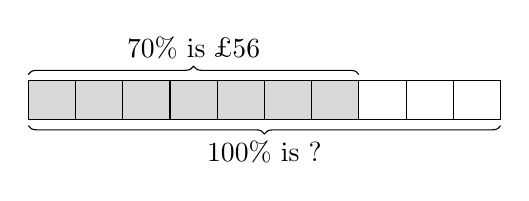
\begin{tikzpicture}[x=6mm,y=5mm]
  \fill[black!15] (0,0) rectangle (7,1);
  \foreach \i in {0,...,9}{\draw (\i,0) rectangle ++(1,1);}
  \draw[decorate,decoration={brace,amplitude=3pt}] (0,1.15) -- (7,1.15) node[midway,above=2pt] {70\% is £56};
  \draw[decorate,decoration={brace,amplitude=3pt,mirror}] (0,-0.15) -- (10,-0.15) node[midway,below=2pt] {100\% is ?};
\end{tikzpicture}
\q After a 10\% increase, a bill is £77. What was the bill before the increase?
\q A price including 20\% VAT is £54. What was the price before VAT was added?
\end{ealglossed}

% ----------------------------------------------------------------
\topic{Problem solving}
\q A £90 coat is on sale in two shops. Shop A takes $\frac13$ off. Shop B takes 30\% off, then a further 5\% off the sale price. Which shop is cheaper, and by how much?
\q Kim says, ``After 30\% off, a bike costs £280, so the original price was $280\times1.3=$ £364.'' Explain Kim's mistake, and find the correct original price.
\begin{ealglossed}
\q Write down three different \ealgloss{fractions}{ułamki} between $\frac35$ and $\frac7{10}$. Show how you know that each one is in this range.
\end{ealglossed}

\end{multicols}

\end{document}